\section{Entrenamiento y resultados}
En esta etapa se entrenó la CNN con el conjunto completo y se evaluó el efecto de reducir el número de imágenes disponibles por clase, comparando subconjuntos aleatorios de fotografías reales con conjuntos sintéticos obtenidos con DM. Después, con el conjunto completo, se probaron variaciones de hiperparámetros. Todas las tablas y figuras de esta sección se generan con el notebook \texttt{reports/entregable\_3/avance3.ipynb} del repositorio público del proyecto \parencite{repositorio} (sección~\ref{sec:notebook}).

\subsection{Diseño de los experimentos}
Se consideraron tres modalidades de entrenamiento. La primera, \textit{conjunto completo}, emplea las 12,753 imágenes reales de entrenamiento y funciona como referencia. La segunda, \textit{aleatorio}, utiliza un subconjunto balanceado de fotografías reales tomadas al azar, con la misma cantidad de imágenes por clase. La tercera, \textit{destilado}, sustituye ese subconjunto por imágenes sintéticas optimizadas con DM. En las dos últimas se evaluaron dos tamaños: una imagen por clase (IPC = 1, 104 imágenes) y diez imágenes por clase (IPC = 10, 1,040 imágenes), que representan reducciones del 99.18\,\% y 91.85\,\% frente al conjunto original.

Las cuatro configuraciones reducidas se entrenaron con las semillas 0, 1 y 2, hasta 300 épocas, evaluando validación cada diez épocas. El conjunto completo se entrenó una vez (semilla 0), hasta 50 épocas, evaluando validación en cada época. En todos los casos se usó el mismo conjunto de validación de 3,712 imágenes reales; los datos de prueba no se usaron para seleccionar modelos.

\subsection{Resultados de clasificación}
La Tabla~\ref{tab:resultados} resume los resultados. Para los conjuntos reducidos se presenta el promedio de las tres semillas y la desviación estándar muestral del F1 macro. La exactitud se incluye como métrica complementaria, pero el F1 macro es la medida principal por el desbalance entre clases.

\begin{table*}[htbp]
\centering
\caption{Resultados de validación y tiempo de entrenamiento de la CNN a $112\times112$. Para los conjuntos reducidos se reportan promedios de tres semillas.}
\label{tab:resultados}
\small
\begin{tabular}{lcccrr}
\toprule
Modalidad & IPC & Corridas & F1 macro & Exactitud (\%) & Entrenamiento (s) \\
\midrule
Aleatorio & 1 & 3 & 0.0514 $\pm$ 0.0029 & 5.75 & 35.4 \\
Destilado (DM) & 1 & 3 & 0.0672 $\pm$ 0.0052 & 9.85 & 36.3 \\
Aleatorio & 10 & 3 & 0.2575 $\pm$ 0.0082 & 25.86 & 329.4 \\
Destilado (DM) & 10 & 3 & 0.2044 $\pm$ 0.0235 & 20.55 & 272.5 \\
Conjunto completo & -- & 1 & 0.5538 & 61.61 & 581.5 \\
\bottomrule

\end{tabular}
\end{table*}

Con una sola imagen por clase, el conjunto destilado alcanzó un F1 macro promedio de 0.0672, frente a 0.0514 con imágenes reales elegidas al azar, una diferencia de 0.0158 a favor de DM. Esto sugiere que, con una reducción extrema, la optimización de las imágenes sintéticas conserva información útil para la clasificación. Con diez imágenes por clase ocurrió lo contrario: la selección aleatoria alcanzó 0.2575 y el conjunto destilado 0.2044, una diferencia de 0.0531 a favor de las fotografías reales (Figura~\ref{fig:comparacion}). Por tanto, la destilación no mostró una ventaja consistente en ambos tamaños.

La CNN entrenada con el conjunto completo obtuvo el mejor resultado: F1 macro de 0.5538 y exactitud de 61.61\,\%. Como el modelo completo se entrenó una sola vez y las demás configuraciones cuentan con tres repeticiones, estas comparaciones son resultados preliminares, no evidencia estadística definitiva.

\begin{figure}[pos=!ht]
\centering
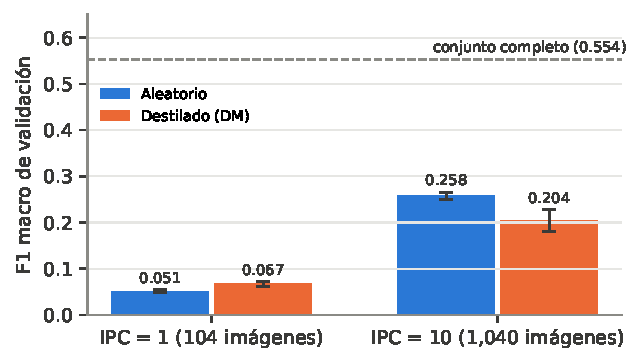
\includegraphics[width=\columnwidth]{comparacion_f1.pdf}
\caption{F1 macro de validación de los subconjuntos aleatorios y destilados. Las barras de error indican una desviación estándar entre tres semillas y la línea discontinua, la corrida con el conjunto completo.}
\label{fig:comparacion}
\end{figure}

\subsection{Costo computacional de la destilación}
La Tabla~\ref{tab:costos} separa el tiempo de entrenamiento del tiempo de destilación. Los tiempos de entrenamiento excluyen las evaluaciones periódicas de validación. La destilación se ejecutó una sola vez por IPC y sus imágenes se reutilizaron en las tres semillas, por lo que no debe contarse una destilación por semilla. La columna ``Total'' suma una destilación al tiempo promedio de entrenamiento; estima el costo de preparar el conjunto sintético y entrenar un modelo con él, pero no incluye la descarga ni la preparación de los datos.

\begin{table}[htbp]
\centering
\caption{Tiempo promedio de entrenamiento y de destilación previa, en segundos.}
\label{tab:costos}
\small
\begin{tabular}{lcrrr}
\toprule
Modalidad & IPC & Entren. & Destil. & Total \\
\midrule
Aleatorio & 1 & 35.4 & -- & 35.4 \\
Destilado (DM) & 1 & 36.3 & 985.4 & 1,021.7 \\
Aleatorio & 10 & 329.4 & -- & 329.4 \\
Destilado (DM) & 10 & 272.5 & 1,510.0 & 1,782.5 \\
Conjunto completo & -- & 581.5 & -- & 581.5 \\
\bottomrule

\end{tabular}
\end{table}

Aunque entrenar con conjuntos reducidos toma menos tiempo que usar las 12,753 fotografías, la destilación incrementa considerablemente el costo inicial: con IPC = 10, preparar y entrenar el conjunto destilado (1,782.5 s) toma más que entrenar con el conjunto completo (581.5 s). Por ello, los resultados no permiten concluir que DM sea más rápido para entrenar un solo modelo; su costo solo podría amortizarse si las mismas imágenes sintéticas se reutilizaran en muchos entrenamientos.

\subsection{Curvas de aprendizaje}
Cada corrida guarda un archivo \texttt{history.csv} con la pérdida y la exactitud de entrenamiento y la pérdida, exactitud y F1 macro de validación por época. Las métricas de entrenamiento se registran durante la época, con aumento de datos y \textit{dropout} activos, mientras que las de validación se calculan al final de la época sin transformaciones. Por eso, al inicio, la exactitud de validación puede ser mayor que la de entrenamiento.

\paragraph{Conjunto completo.} La Figura~\ref{fig:curvas_completo} muestra que las pérdidas de entrenamiento y validación bajan juntas hasta la época 21 (de 3.94 y 3.59 a 1.69 y 1.74). A partir de la época 25 se separan: la de entrenamiento sigue bajando hasta 1.07, mientras que la de validación se estanca entre 1.51 y 1.69. La exactitud muestra lo mismo: al final, la de entrenamiento llega a 68.1\,\% y la de validación se queda en 62.6\,\%. Es el inicio del sobreajuste, aunque moderado, porque el F1 de validación todavía mejora lentamente hasta la época 38 (0.5538), que coincide con la menor pérdida de validación (1.510). En las cinco épocas siguientes el F1 no mejoró, y la parada temprana detuvo el entrenamiento en la época 43. El \textit{checkpoint} guardado corresponde a la época 38, así que el modelo reportado no incluye las épocas en las que empezaba a sobreajustar.

\begin{figure*}[htbp]
\centering
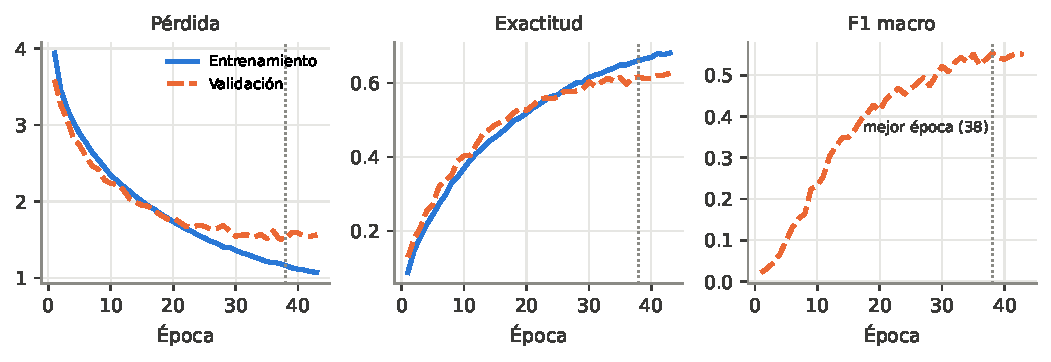
\includegraphics[width=0.9\textwidth]{curvas_completo.pdf}
\caption{Curvas de aprendizaje con el conjunto completo: pérdida y exactitud de entrenamiento frente a validación, y F1 macro de validación. La línea punteada marca la mejor época (38), cuyo modelo se guardó.}
\label{fig:curvas_completo}
\end{figure*}

\paragraph{Conjuntos reducidos.} En la Figura~\ref{fig:curvas_reducidos}, el sobreajuste es mucho más marcado. Con IPC = 10, la exactitud de entrenamiento llega a 70--85\,\% y la pérdida de entrenamiento baja a 0.5--0.9, pero la exactitud de validación se estanca alrededor de 25\,\% (aleatorio) y 19\,\% (destilado). La pérdida de validación alcanza su mínimo entre las épocas 30 y 50 (alrededor de 3.6--3.9) y luego crece hasta 7.4--9.3, es decir, la red memoriza las 1,040 imágenes. Con IPC = 1 ocurre lo mismo con mayor intensidad: la validación queda entre 5 y 10\,\% de exactitud y su pérdida sube hasta 12--18. El conjunto destilado con IPC = 1 se ajusta más lentamente (exactitud de entrenamiento final de 57--63\,\%, contra 62--83\,\% del aleatorio), lo que concuerda con que sus imágenes sintéticas resumen la clase en lugar de ser ejemplos fáciles de memorizar.

Aunque la pérdida de validación crece, el mejor F1 de los conjuntos reducidos se alcanza tarde (entre las épocas 170 y 280). Esto pasa porque la pérdida castiga las predicciones equivocadas hechas con mucha confianza, mientras que el F1 solo depende de la clase predicha: el modelo sigue acertando algunas imágenes más, pero se vuelve muy confiado en sus errores. Por eso conviene seleccionar el modelo por F1 y no por la pérdida.

\begin{figure*}[htbp]
\centering
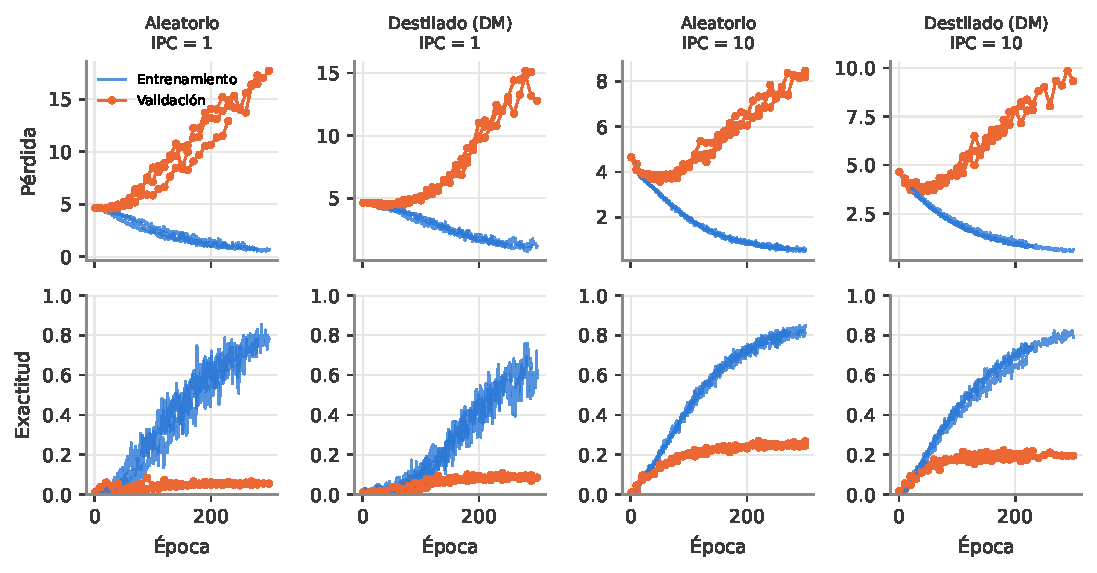
\includegraphics[width=0.95\textwidth]{curvas_reducidos.pdf}
\caption{Curvas de aprendizaje de los conjuntos reducidos (tres semillas por configuración). Validación se evaluó cada diez épocas; los marcadores indican las épocas evaluadas.}
\label{fig:curvas_reducidos}
\end{figure*}

\subsection{Experimentos de hiperparámetros con el conjunto completo}
Para estudiar los hiperparámetros, se tomó como referencia una política de entrenamiento con AdamW (\textit{weight decay} de 0.01), tasa de aprendizaje inicial de $10^{-3}$ que se reduce a la mitad cuando la pérdida de validación se estanca, \textit{dropout} de 0.5, aumento de datos, lotes de 64 y paciencia de 12 épocas. A partir de ella se cambió \textbf{un solo factor} en cada experimento: la tasa de aprendizaje ($3\times10^{-4}$), el \textit{dropout} (0.3) y la regularización en conjunto (sin \textit{dropout}, sin aumento de datos y sin \textit{weight decay}). En estas corridas, las métricas de entrenamiento se miden sobre 3,712 imágenes fijas de entrenamiento sin aumentos ni \textit{dropout}, igual que validación, por lo que la brecha entre ambas sí mide el sobreajuste. Los resultados están en la Tabla~\ref{tab:hiperparametros} y la Figura~\ref{fig:curvas_hp}.

\begin{table*}[htbp]
\centering
\caption{Efecto de los hiperparámetros con el conjunto completo (una semilla). La brecha es el F1 de entrenamiento menos el de validación en la mejor época.}
\label{tab:hiperparametros}
\small
\begin{tabular}{lrrrrc}
\toprule
Configuración & F1 val. & Exactitud val. (\%) & F1 entren. & Brecha & Mejor época / épocas \\
\midrule
Referencia (LR $10^{-3}$, dropout 0.5) & 0.5784 & 64.06 & 0.814 & 0.235 & 91 / 103 \\
Tasa de aprendizaje $3\times10^{-4}$ & 0.4605 & 54.18 & 0.554 & 0.094 & 98 / 110 \\
Dropout 0.3 & 0.5596 & 61.96 & 0.816 & 0.256 & 61 / 73 \\
Sin dropout, aumento ni weight decay & 0.5332 & 59.64 & 0.877 & 0.344 & 34 / 46 \\
\bottomrule

\end{tabular}
\end{table*}

\begin{figure*}[htbp]
\centering
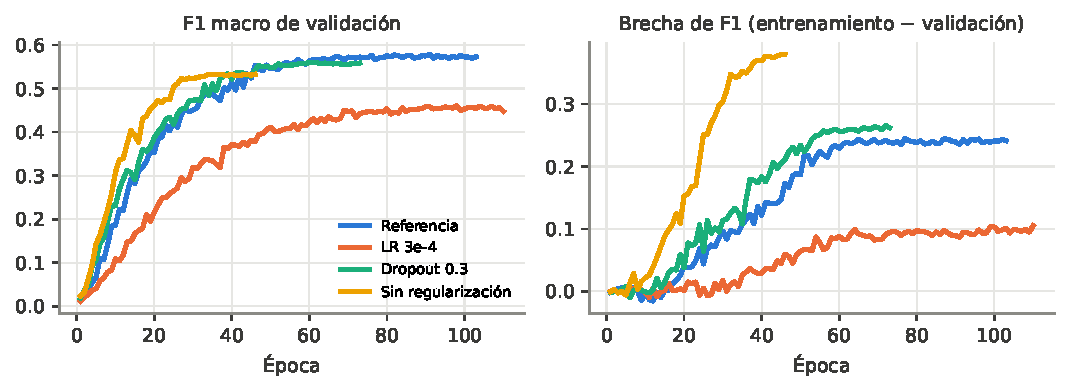
\includegraphics[width=0.9\textwidth]{curvas_hiperparametros.pdf}
\caption{F1 macro de validación y brecha de F1 entre entrenamiento y validación por época para cada configuración de hiperparámetros.}
\label{fig:curvas_hp}
\end{figure*}

\paragraph{Tasa de aprendizaje.} Reducir la tasa de $10^{-3}$ a $3\times10^{-4}$ bajó el F1 de 0.5784 a 0.4605. La brecha es la más pequeña (0.094), pero el F1 de entrenamiento también es bajo (0.554): el modelo no está sobreajustando, está \textbf{subajustando}. Con pasos más pequeños, la red aprende más lento y la reducción automática de la tasa la lleva al mínimo ($10^{-5}$) antes de converger, así que después de 110 épocas sigue lejos de la referencia. Con este presupuesto de épocas, $10^{-3}$ es la mejor opción.

\paragraph{Dropout.} Bajar el \textit{dropout} de 0.5 a 0.3 redujo el F1 a 0.5596 y aumentó ligeramente la brecha (de 0.235 a 0.256). La menor pérdida de validación también empeoró (de 1.464 a 1.596). Con menos neuronas apagadas, la capa densa memoriza un poco más, así que conviene mantener 0.5.

\paragraph{Regularización.} Sin \textit{dropout}, sin aumento de datos y sin \textit{weight decay}, la red converge más rápido (mejor época 34 de 46), pero alcanza la brecha más grande (0.344): el F1 de entrenamiento llega a 0.877, mientras que el de validación se queda en 0.5332. Es el caso más claro de \textbf{sobreajuste}, lo que confirma que la regularización es la responsable de la mejora de la referencia.

La referencia (F1 de 0.5784, exactitud de 64.06\,\%) supera a la corrida original del Avance 3 (0.5538). Sin embargo, como esa política cambia varios factores a la vez (optimizador, reducción de la tasa, tamaño de lote y paciencia), la mejora no puede atribuirse a uno solo. No se evaluó el tamaño de imagen; queda como siguiente experimento, por ejemplo $160\times160$.

\subsection{Notebook y reproducibilidad}
\label{sec:notebook}
El notebook \texttt{reports/entregable\_3/avance3.ipynb} del repositorio \url{https://github.com/Lunaaaalj/NeuralNetworksTeamEnvironment} reproduce esta sección de principio a fin: descarga y revisión de los datos, construcción de la CNN, entrenamiento de todas las configuraciones (activando \texttt{RUN\_TRAINING}), re-evaluación de los modelos guardados, generación de las Tablas~\ref{tab:resultados}, \ref{tab:costos} y~\ref{tab:hiperparametros} y de todas las figuras de curvas. La configuración exacta del Avance 3 está en \texttt{config\_avance3.yaml} y la de cada experimento de hiperparámetros, junto con su historial, en \texttt{hiperparametros/}. Al re-evaluar los 13 modelos guardados sobre las 3,712 imágenes de validación, el F1 macro y la exactitud coincidieron exactamente con los registrados durante el entrenamiento.

\subsection{Limitaciones y siguientes pasos}
El tamaño y la composición del conjunto de entrenamiento influyen mucho en el desempeño de la CNN. DM mejoró a la selección aleatoria con una imagen por clase, pero no con diez, y el costo de crear las imágenes sintéticas superó el de entrenar con ellas. Con el conjunto completo, la regularización (\textit{dropout} de 0.5, aumento de datos y \textit{weight decay}) y una tasa de aprendizaje de $10^{-3}$ dieron el mejor resultado.

Las conclusiones están limitadas a una arquitectura, una resolución de $112\times112$, una sola semilla en los experimentos con el conjunto completo y al conjunto de validación, ya que las etiquetas de prueba no están disponibles. Los siguientes pasos son probar resoluciones mayores, repetir los experimentos de hiperparámetros con varias semillas y estudiar qué clases son más difíciles de reconocer.
